\documentclass{beamer} 
\usepackage{amsmath,amsthm,amsfonts}
\usepackage{graphicx,microtype,parskip}
\usepackage{caption,subcaption,multirow}
\usepackage{attrib}

\frenchspacing

\usetheme{default}
\usecolortheme{whale}

\setbeamertemplate{navigation symbols}{}

\setbeamercolor{title}{fg=blue,bg=white}

\setbeamercolor{block title}{fg=white,bg=gray}
\setbeamercolor{block body}{fg=black,bg=lightgray}

\setbeamercolor{block title alerted}{fg=white,bg=darkgray}
\setbeamercolor{block body alerted}{fg=black,bg=lightgray}

\let\Tiny\tiny% http://tex.stackexchange.com/q/58087/5764

\setbeamertemplate{footline} {
  \hbox{\begin{beamercolorbox}[wd=1\paperwidth,ht=2.25ex,dp=1ex,right]{framenumber}%
    \usebeamerfont{framenumber}\insertframenumber{} / \inserttotalframenumber\hspace*{2ex}
  \end{beamercolorbox}}%
  \vskip0pt%
}

\begin{document}


\begin{frame}
  \begin{columns}
    \begin{column}{0.5\textwidth}
      \begin{center}
        \includegraphics[height=0.8\textheight,width=\textwidth,keepaspectratio=true]{figure/stanley_macro}
      \end{center}
    \end{column}
    \begin{column}{0.5\textwidth}
      \begin{center}
        \includegraphics[height=0.8\textheight,width=\textwidth,keepaspectratio=true]{figure/brown_macro}
      \end{center}
    \end{column}
  \end{columns}
\end{frame}

\begin{frame}
  \frametitle{Core disciplines}
  \begin{definition}
    \begin{itemize}
      \item \alert{macroevolution}: study of patterns which emerge when considering the evolutionary history of multiple species.
      \item \alert{macroecology}: study of patterns which emerge when considering the ecology of multiple species.
      \item \emph{in both time and space}
    \end{itemize}
  \end{definition}
\end{frame}

\begin{frame}
  \frametitle{Traits as conceptual and operational link}

  \begin{definition}
    \begin{itemize}
      \item \alert{trait}: identifiable property of an organism \\e.g. pelage color, body mass, beak depth, tooth shape
      \item \alert{functional trait}: trait that strongly influences performance/means of interacting with environment
      \item \alert{species trait}: identifiable property assignable to a species
    \end{itemize}
  \end{definition}
\end{frame}






\begin{frame}
  \begin{alertblock}{Why does extinction risk vary between taxa?}
    \begin{itemize}
      \item How do traits shape these differences?
      \item How do the effect of traits on duration (\alert{extinction selectivity}) vary with expected duration (\alert{extinction intensity})?
      \item How do shared time of origination or evolutionary history relate to extinction risk?
      \item Is species extinction risk age-independent?
    \end{itemize}
  \end{alertblock}
\end{frame}


\begin{frame}
  \frametitle{Extinction}
  \begin{block}{Simpson 2016 \em{bioRxiv}}
    \begin{quote}
      Population decline maybe a common cause of \dots extinction, but organisms never die from population decline, and population decline is never caused by organismal death alone \dots It's the relative balance between birth, death, and lifespan of organisms that determines \dots extinction. 
    \end{quote}
  \end{block}
\end{frame}

\begin{frame}
  \frametitle{Species selection}

  \begin{block}{Rabosky and McCune 2010 \em{TREE}}
    \begin{quote}
      Species selection is the outcome of heritable variation in speciation and extinction rates among taxa.
    \end{quote}
  \end{block}

%  \begin{itemize}
%    \item avoids selection versus sorting, \\``strict'' species selection versus effect macroevolution
%  \end{itemize}
\end{frame}

\begin{frame}
  \frametitle{Species fitness}

  \begin{block}{Cooper 1984 \em{J. Theoretical Biology}}
    Expected time till extinction.
  \end{block}


  \begin{itemize}
    \item \alert{logic:} if more fit, more likely to be present/``living''
    \item distribution based definition (i.e. population level)
    \item other definitions can be derived based on definition of extinction
  \end{itemize}

\end{frame}

\begin{frame}
  \frametitle{Law of Constant Extinction}

  \begin{block}{Van Valen 1973 \em{Evol. Theory}}
    Extinction risk (species fitness), in a given adaptive zone, is taxon--age independent.
  \end{block}

  \begin{center}
    \includegraphics[width = \textwidth,height = 0.5\textheight,keepaspectratio = true]{figure/surv_sim}

  \end{center}

\end{frame}

\begin{frame}
  \frametitle{Survival of the unspecialized}
  \begin{block}{Simpson 1944 \em{Tempo and Mode in Evolution} p. 143}
    \begin{quote}
      When related phyla die out \dots more specialized phyla tend to become extinct before less specialized. This phenomenon is also far from universal, but it is so common that it does deserve recognition as a rule or principle in evolutionary studies: \textbf{the rule of the survival of the relatively unspecialized.}
    \end{quote}
  \end{block}
\end{frame}




\begin{frame}
  \begin{alertblock}{What shapes the functional diversity of a species pool?}
    \begin{itemize}
      \item When are functional groups enriched or depleted in a species pool? 
      \item How does environmental context affect functional diversity?
      \item Does origination or extinction more strongly shape functional diversity?
    \end{itemize}
  \end{alertblock}
\end{frame}

\begin{frame}
  \frametitle{Species pool concept}

  \begin{center}
    \includegraphics[height=0.8\textheight,width=\textwidth,keepaspectratio=true]{figure/schemske_pool}
  \end{center}

  \tiny{\attrib{Mittelbach and Schemske 2015 \em{TREE}}}
\end{frame}

\begin{frame}
  \frametitle{Functional groups}

  \begin{center}
    \includegraphics[height=0.8\textheight,width=\textwidth,keepaspectratio=true]{figure/ecocube}
  \end{center}

  \tiny{\attrib{Bambach \em{et al.} 2007 \em{Palaeontology}}}
\end{frame}

\begin{frame}
  \frametitle{Functional groups over time}

  \begin{center}
    \includegraphics[height=0.8\textheight,width=\textwidth,keepaspectratio=true]{figure/bush_cube_time}
  \end{center}

  \tiny{\attrib{Bush and Bambach 2011 \em{Annu. Rev. Earth Planet Sci.}}}
\end{frame}


\begin{frame}
  \begin{alertblock}{How do we ask and ``answer'' these questions?}
    \begin{itemize}
      \item Represent our scientific questions in statistical statements
      \item ``Handle'' complicating factors
        \begin{itemize}
          \item preservation and other forms of incomplete observation
          \item autocorrelation: time, phylogeny, geography
        \end{itemize}
      \item Prediction 
    \end{itemize}
  \end{alertblock}
\end{frame}


\begin{frame}
  \frametitle{Structured data in biology and paleontology}

  \begin{center}
    \includegraphics[width = \textwidth,height = 0.8\textheight,keepaspectratio = true]{figure/ovaskainen_data}
  \end{center}

  \tiny{\attrib{Ovaskainen \textit{et al.} 2017 \em{Ecology Letters}}}
\end{frame}

\begin{frame}
  \frametitle{Bayesian inference and statistics}

  \begin{columns}
    \begin{column}{0.5\textwidth}
      \begin{itemize}
        \item flexible, expressive, intuitive
        \item regularize, partial pooling, external information
        \item Stan probabilistic programming language
          \begin{itemize}
            \item Hamiltonian Monte Carlo
            \item Automatic Differentiation Variational Inference
          \end{itemize}
      \end{itemize}
    \end{column}
    \begin{column}{0.5\textwidth}
      \begin{center}
        \includegraphics[width = \textwidth,height = 0.8\textheight,keepaspectratio = true]{figure/bda_cover}
      \end{center}
    \end{column}
  \end{columns}
\end{frame}

\begin{frame}
  \frametitle{Models of structured data}

  \begin{center}
    \includegraphics[width = \textwidth,height = 0.8\textheight,keepaspectratio = true]{figure/ovaskainen_dag}
  \end{center}

  \tiny{\attrib{Ovaskainen \textit{et al.} 2017 \em{Ecology Letters}}}
\end{frame}

%\begin{frame}
%  \frametitle{Mammals and brachiopods}
%
%  \begin{columns}
%    \begin{column}{0.5\textwidth}
%      \begin{center}
%        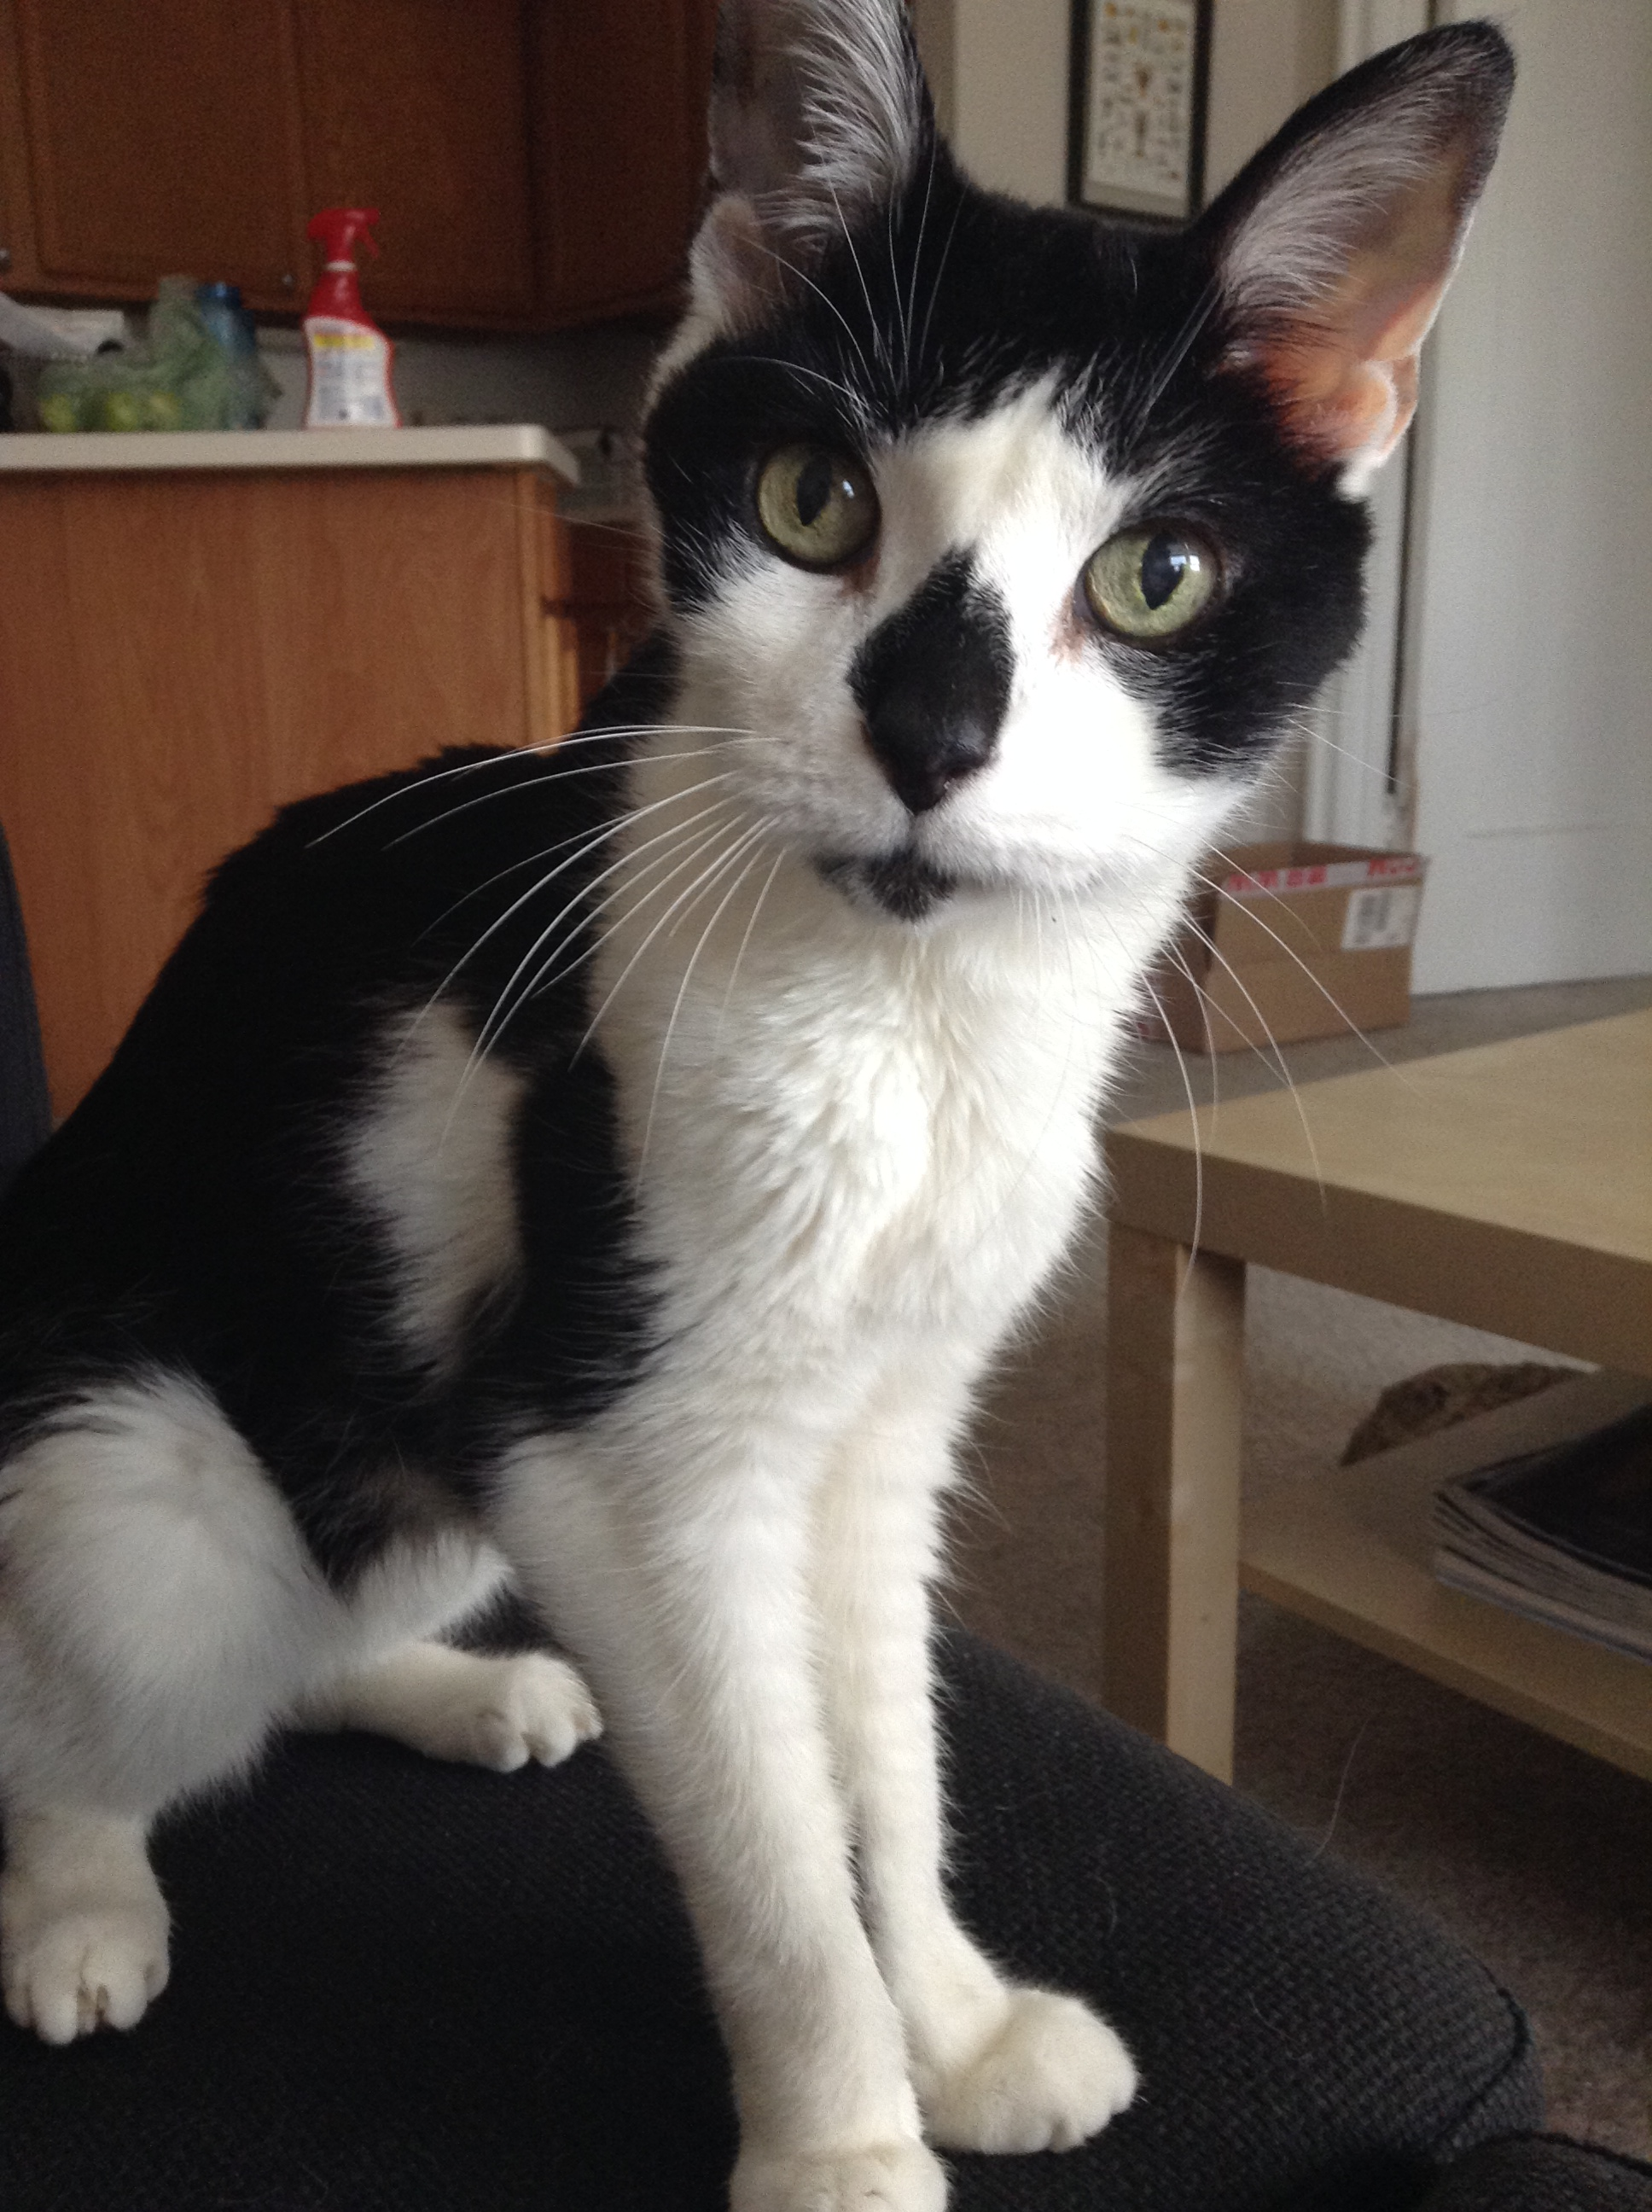
\includegraphics[height = 0.6\textheight, keepaspectratio = true]{figure/monty}
%      \end{center}
%    \end{column}
%    \begin{column}{0.5\textwidth}
%      \begin{center}
%        \includegraphics[height = 0.6\textheight, keepaspectratio = true]{figure/tattoo}
%      \end{center}
%    \end{column}
%  \end{columns}
%\end{frame}


\end{document}
